\section{Алгоритмы, основанные на отношении доминирования.}
\begin{figure}[h]
Решения ранжируются в соответствии с относительным местоположением в
пространстве критериев\\
Dominance rank: сколько решений доминируют текущее?\\
Алгоритмы: MOGA, NPGA
Из пространства критериев выбираются доминантные решения, удовлетворяющие  значениям критериев, благодаря этому и dominance rank можно определить область множества доминирующих решений.
\begin{center}
    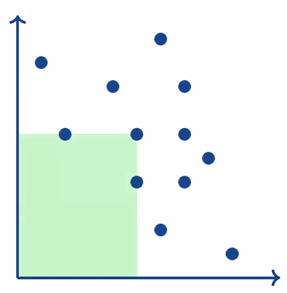
\includegraphics[width=0.8\linewidth]{images/Dominate_1.PNG}
    \caption{Пример когда выбираем текущее решение (объект) ТОЛЬКО ПОТОМ составляем множество(субъекты) которое доминирует над заданным}
    \label{fig:mpr}
\end{center}
\end{figure}

\begin{figure}[!ht]
Решения ранжируются в соответствии с относительным местоположением в
пространстве критериев
Dominance count: сколько решений доминирует текущее?
Алгоритмы: SPEA, SPEA2
\begin{center}
    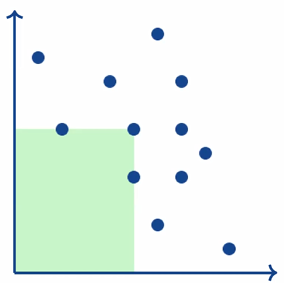
\includegraphics[width=1.2\linewidth]{images/Dominate_2.PNG}
    \caption{Пример когда СНАЧАЛА выбираем множество(объекты в данном случае) решений и ТОЛЬКО ПОТОМ находим доминирующие над этим множеством решения(субъект}
    \label{fig:mpr}
\end{center}
\end{figure}

\begin{figure}[!ht]
Решения ранжируются в соответствии с относительным местоположением в
пространстве критериев
Dominance depth: на каком фронте (Фронт Парето) расположено текущее решение?
Алгоритмы: NSGA, NSGA-II, NSGA-III, ...\\

Составляется набор значений, по которому определяется доминирующее решение. В процессе выбора доминирующих критериев выставляются наборы доминантных подмножеств решений. Эти решения обладают сопоставимым набором векторов доминантных критериев
\begin{center}
    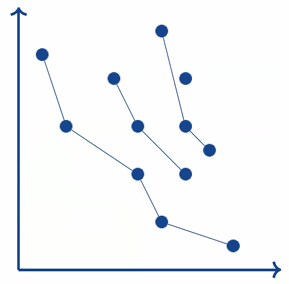
\includegraphics[width=0.8\linewidth]{images/Dominate_3.PNG}
    \caption{Пример с фронтом Парето}
    \label{fig:mpr}
\end{center}
\end{figure}

\newpage
Simple Evolutionary Multiobjective Optimizer (SEMO)\\
Поддерживаем популяцию недоминированных решений ( на всём итеративном процессе)\\
На каждой итерации:\\
- Генерируем одно новое решение (с использованием операторов
мутации, скрещивания и т.д.)\\
- Если оно не доминируется ни одним решением из популяции,
добавляем его в популяцию\\
- Если какие-то решения в популяции доминируются новым решением,
удаляем эти решения из популяции\\

Особенности:\\
$(+)$ Весьма прост для теоретического анализа и для реализации\\
(-) Экстремальный элитизм: может застрять на неоптимальном фронте (Все особи проходят на глобальный оптимум(ничего не удаляется)). Это говорит о том, что итеративный процесс выродился на данном этапе. Может произойти на этапе формирования фронта Парето (формирования векторов), когда значения критериев близки к друг другу или что еще хуже если эдентичны. То есть сам фронт будет состоять только из одного вектора\\
(-) Популяция может неконтролируемо разрастаться\\
Еще одна причина застревания в локальном оптимуме.

